\section{Polynomial Regression}


\begin{frame}{Learning outcomes}
    \begin{itemize}
        \item Recognize a non-linear relationship from a scatter plot and from a residual plot
        \item Fit polynomial regression as an ordinary linear regression that uses the powers of $x$ as columns of the design matrix
        \item Interpret a polynomial fit through the slope of the fitted curve and its turning point
        \item Choose the degree with nested-model $F$-tests and judge the risks: collinearity of powers, extrapolation, overfitting
        \item Use other transformations of the features ($\log x$, $\sqrt{x}$) within the same framework
    \end{itemize}
\end{frame}


\begin{frame}[allowframebreaks]{When a straight line is not enough}
    \begin{itemize}
        \item Auto data: fuel economy (mpg) against engine power (horsepower) for $n = 392$ cars
        \item The scatter plot is curved: mpg falls quickly at low horsepower and levels off at high horsepower
        \item The straight-line fit has $R^2 = 0.606$, but its residuals show a U-shape: they are positive at both ends of the fitted range and negative in the middle, so the line under-predicts at the extremes and over-predicts in between
        \item A systematic pattern in the residuals means the model has missed structure that the data contain
    \end{itemize}
    \begin{center}
        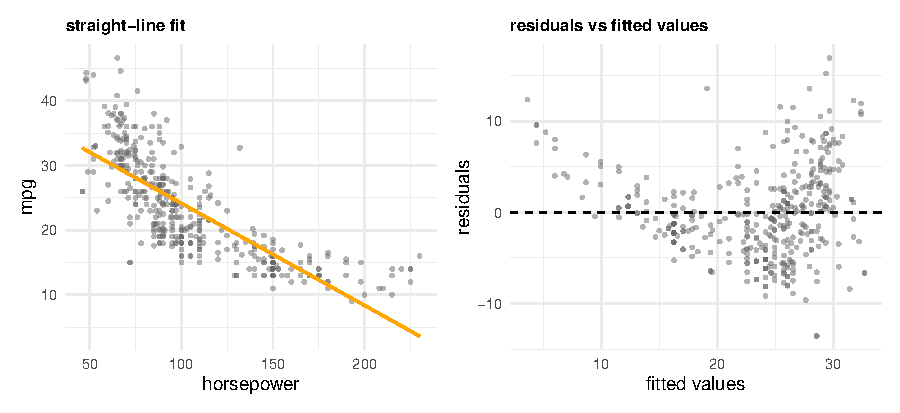
\includegraphics[width=0.95\linewidth]{figures/reg_auto_scatter.pdf}
    \end{center}
\end{frame}


\begin{frame}{The polynomial regression model}
    \begin{itemize}
        \item \textbf{Polynomial regression} adds powers of the feature: $y = \beta_0 + \beta_1 x + \beta_2 x^2 + \dots + \beta_d x^d + \varepsilon$; $d$ is the \emph{degree}
        \item It is still a \emph{linear} regression: the model is linear in the coefficients $\beta_0, \dots, \beta_d$; the columns $x, x^2, \dots, x^d$ are simply treated as $d$ separate features
        \item Any continuous curve on a bounded interval can be approximated arbitrarily well by a polynomial of high enough degree (Weierstrass theorem), so polynomials are a flexible family
        \item Degree 1 is a line, degree 2 a parabola (one bend), degree 3 an S-shape (up to two bends); a degree-$d$ polynomial has at most $d-1$ bends
    \end{itemize}
\end{frame}


\begin{frame}{Ordinary least squares still applies}
    \begin{itemize}
        \item Only the columns of the design matrix change; the first cars in the Auto data (horsepower 130, 165, 150 and mpg 18, 15, 18) give, for $d = 2$:
    \end{itemize}
    \[
        \tilde{\mathbf{X}} = \begin{bmatrix} 1 & x^{(1)} & (x^{(1)})^2 \\ 1 & x^{(2)} & (x^{(2)})^2 \\ 1 & x^{(3)} & (x^{(3)})^2 \\ \vdots & \vdots & \vdots \end{bmatrix} = \begin{bmatrix} 1 & 130 & 16900 \\ 1 & 165 & 27225 \\ 1 & 150 & 22500 \\ \vdots & \vdots & \vdots \end{bmatrix}, \qquad \mathbf{y} = \begin{bmatrix} 18 \\ 15 \\ 18 \\ \vdots \end{bmatrix}
    \]
    \begin{itemize}
        \item The normal equations, $\hat{\symbf{\beta}} = (\tilde{\mathbf{X}}^\top \tilde{\mathbf{X}})^{-1} \tilde{\mathbf{X}}^\top \mathbf{y}$, and everything derived from them carry over: standard errors, $t$-tests, the $F$-test, ANOVA, confidence and prediction intervals, residual diagnostics
        \item The powers of $x$ are functions of the same variable, so features cannot be changed one at a time: "holding the other features fixed" has no meaning for $x$ and $x^2$
    \end{itemize}
\end{frame}


\begin{frame}{The quadratic fit}
    \begin{center}
        \small
        \begin{tabular}{lrrrr}
            \toprule
            & coefficient & std. error & $t$-statistic & $p$-value \\
            \midrule
            intercept & 56.9001 & 1.8004 & 31.60 & $<0.0001$ \\
            horsepower & $-0.46619$ & 0.03112 & $-14.98$ & $<0.0001$ \\
            horsepower$^2$ & 0.001231 & 0.000122 & 10.08 & $<0.0001$ \\
            \bottomrule
        \end{tabular}
    \end{center}
    \begin{itemize}
        \item $\widehat{\text{mpg}} = 56.90 - 0.4662\,\text{hp} + 0.001231\,\text{hp}^2$, with $R^2 = 0.688$ (linear fit: 0.606) and $\mathrm{RSE} = 4.37$ (linear fit: 4.91)
        \item The overall $F$-test gives $F = 428.0$ on $(2, 389)$ degrees of freedom, $p < 0.0001$
        \item The quadratic term is highly significant ($t = 10.08$): the curvature is real, not noise
    \end{itemize}
\end{frame}


\begin{frame}{Interpreting a polynomial}
    \begin{itemize}
        \item The effect of the feature depends on its own value: for the quadratic fit the slope is $\partial \hat{y} / \partial x = \hat\beta_1 + 2 \hat\beta_2 x$, like an interaction of $x$ with itself
        \item Auto: the slope is $-0.343$ mpg per horsepower at 50 hp, $-0.220$ at 100 hp, $-0.097$ at 150 hp and $+0.100$ at 230 hp: extra power costs less and less mileage, and eventually the fit turns upward
        % \item The fitted parabola has its minimum at the \textbf{turning point} $x^* = -\hat\beta_1 / (2\hat\beta_2) = 189.4$ hp, where the predicted mpg is 12.7
        \item $\hat\beta_2 > 0$ means the curve is convex (U-shaped), $\hat\beta_2 < 0$ concave (hill-shaped); individual coefficients such as $\hat\beta_1 = -0.466$ are not the effect of a one-unit change in $x$
        \item Individual coefficients such as $\hat\beta_1 = -0.466$ are not the effect of a one-unit change in $x$
    \end{itemize}
\end{frame}


\begin{frame}[allowframebreaks]{Polynomial fits on the Auto data}
    \begin{itemize}
        \item $R^2$ is 0.606 for the linear fit, 0.688 for the quadratic and 0.697 for degree 5: the quadratic term helps a lot, further terms barely
        \item The linear fit leaves a U-shaped pattern in the residuals, a systematic structure it failed to capture; for the quadratic fit the U-shape is gone
        \item Higher degrees always improve the fit to the training data, but degree 5 starts to wiggle at the ends: too much flexibility is a risk (bias-variance trade-off, later)
    \end{itemize}
    \begin{center}
        
\includegraphics[width=0.95\linewidth]{figures/reg_auto_poly.pdf}
    \end{center}
\end{frame}


\begin{frame}{Choosing the degree with nested F-tests}
    \begin{center}
        \small
        \begin{tabular}{crrrrr}
            \toprule
            degree $d$ & RSS & $R^2$ & adjusted $R^2$ & $F$ vs degree $d-1$ & $p$-value \\
            \midrule
            1 & 9385.9 & 0.6059 & 0.6049 & & \\
            2 & 7442.0 & 0.6876 & 0.6860 & 101.6 & $<0.0001$ \\
            3 & 7426.4 & 0.6882 & 0.6858 & 0.82 & 0.367 \\
            4 & 7399.5 & 0.6893 & 0.6861 & 1.41 & 0.236 \\
            5 & 7223.4 & 0.6967 & 0.6928 & 9.41 & 0.0023 \\
            \bottomrule
        \end{tabular}
    \end{center}
    \begin{itemize}
        \item Each row tests $H_0\colon \beta_d = 0$ with the partial $F$-test $F = (\mathrm{RSS}_{d-1} - \mathrm{RSS}_d)/(\mathrm{RSS}_d/(n-d-1))$, which equals the squared $t$-statistic of the degree-$d$ term
        \item Going from degree 1 to 2 removes 21\% of the RSS; degrees 3 and 4 add nothing significant; the degree-5 term has $p = 0.0023$
    \end{itemize}
\end{frame}


\begin{frame}{Which degree? Significance is not usefulness}
    \begin{itemize}
        \item A stopping rule ``add terms until the first non-significant one'' picks degree 2; but the degree-5 term is significant after two non-significant ones, and adjusted $R^2$ is highest at degree 5 (0.6928)
        \item Yet degree 5 lowers the RSS by only 2.4\% and raises $R^2$ by only 0.007, and its curve wiggles at the ends of the data
        \item With $n = 392$ even small improvements can be significant, and several tests are run on the same data
        \item In-sample criteria alone cannot settle the degree; combine them with the fitted curve and residual plots, and evaluate on new data (later lecture)
    \end{itemize}
\end{frame}


\begin{frame}{Collinearity among the powers}
    \begin{itemize}
        \item $x$ and $x^2$ move together: in the Auto data $\mathrm{cor}(\text{hp}, \text{hp}^2) = 0.983$ and both have $\mathrm{VIF} = 29.3$, well above the warning level of 5 to 10
        \item \textbf{Centering} the feature removes most of this: with $\tilde{x} = \text{hp} - 104.47$ (the mean), $\mathrm{cor}(\tilde{x}, \tilde{x}^2) = 0.663$ and $\mathrm{VIF} = 1.78$
        \item The fit itself does not change (same $R^2$, RSE and fitted values, same $\hat\beta_2 = 0.001231$); the intercept becomes the predicted mpg at the mean horsepower (21.63) and $\hat\beta_1 = -0.2091$ (SE 0.0077) becomes the slope at the mean horsepower
        \item \textbf{Orthogonal polynomials}: go one step further and make the columns exactly uncorrelated; the fitted curve is the same, but the individual coefficients are no longer interpretable
        \item Raw powers also cause numerical problems (the values of $x^5$ reach $6 \times 10^{11}$ here), another reason to center or use orthogonal polynomials
    \end{itemize}
\end{frame}


\begin{frame}{Other transformations of the features}
    \begin{center}
        \small
        \begin{tabular}{lcc}
            \toprule
            model for mpg & parameters & $R^2$ \\
            \midrule
            hp & 2 & 0.606 \\
            $\log(\text{hp})$ & 2 & 0.668 \\
            $\sqrt{\text{hp}}$ & 2 & 0.644 \\
            $1/\text{hp}$ & 2 & 0.667 \\
            hp $+$ hp$^2$ & 3 & 0.688 \\
            \bottomrule
        \end{tabular}
    \end{center}
    \begin{itemize}
        \item Any fixed function of a feature can be a column of $\tilde{\mathbf{X}}$ ($\log x$, $\sqrt{x}$, $1/x$, $x^2$, \dots): the model stays linear in the coefficients
        \item A one-parameter transformation such as $\log(\text{hp})$ captures much of the curvature with one coefficient fewer than a quadratic
        \item Choose among candidates with residual plots and subject-matter knowledge, not $R^2$ alone
    \end{itemize}
\end{frame}


\begin{frame}[allowframebreaks]{Extrapolation and overfitting}
    \begin{itemize}
        \item A polynomial is a global curve, and outside the range of the data it can behave wildly: the Auto data end at 230 hp, yet the quadratic fit predicts 27.8 mpg at 300 hp (more than at 100 hp: 22.6) and the degree-5 fit predicts 278 mpg
        \item Each added power makes the curve more flexible and lowers the training error, whether or not the new term reflects reality: this is \textbf{overfitting}, the fit follows noise
        \item Degree 5 already turns twice inside the data range and rises at the right end; ISLP notes that polynomial degrees above 3 or 4 are rarely used
        \item Deciding how much flexibility the data support requires new data or resampling: bias-variance trade-off, validation and cross-validation (later lectures)
    \end{itemize}
    \begin{center}
        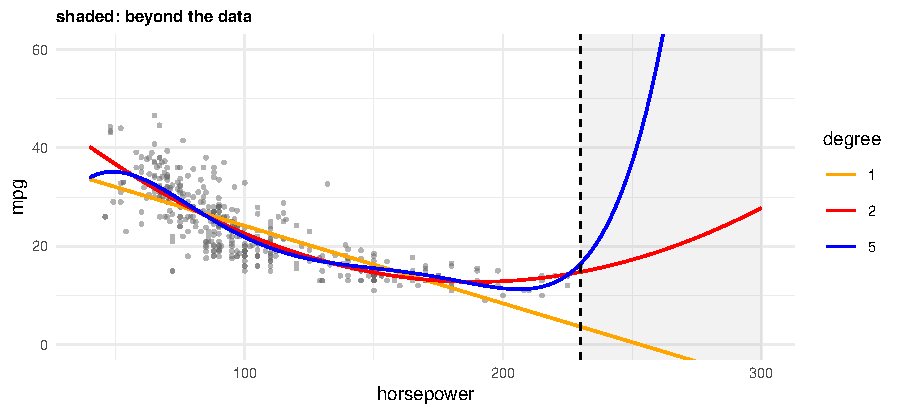
\includegraphics[width=0.95\linewidth]{figures/reg_poly_extrap.pdf}
    \end{center}
\end{frame}


\section{Summary}


\begin{frame}{Summary}
    \begin{itemize}
        \item \textbf{Non-linearity} shows up as a pattern in the residuals; polynomial regression $y = \beta_0 + \beta_1 x + \dots + \beta_d x^d + \varepsilon$ is a linear regression on the design matrix with columns $1, x, \dots, x^d$
        \item \textbf{Interpretation}: the effect of $x$ depends on $x$ itself (slope $\hat\beta_1 + 2\hat\beta_2 x$ for $d = 2$)%; turning point $-\hat\beta_1/(2\hat\beta_2)$
        \item \textbf{Degree}: nested $F$-tests, adjusted $R^2$ and residual plots guide the choice, but they are in-sample tools
        \item \textbf{Cautions}: collinearity of powers (center or use orthogonal polynomials), extrapolation, overfitting
        \item \textbf{Other transformations}: $\log x$, $\sqrt{x}$, $1/x$ fit the same framework
    \end{itemize}
\end{frame}